%% AMS-LaTeX Created with the Wolfram Language : www.wolfram.com

\documentclass[main.tex]{subfiles}
%\documentclass{article}
%\usepackage{amsmath, amssymb, graphics, setspace, parskip}
%\usepackage{graphicx}


%\newcounter{mathematicapage}
\begin{document}

%%%

% \begin{figure}[h]
%     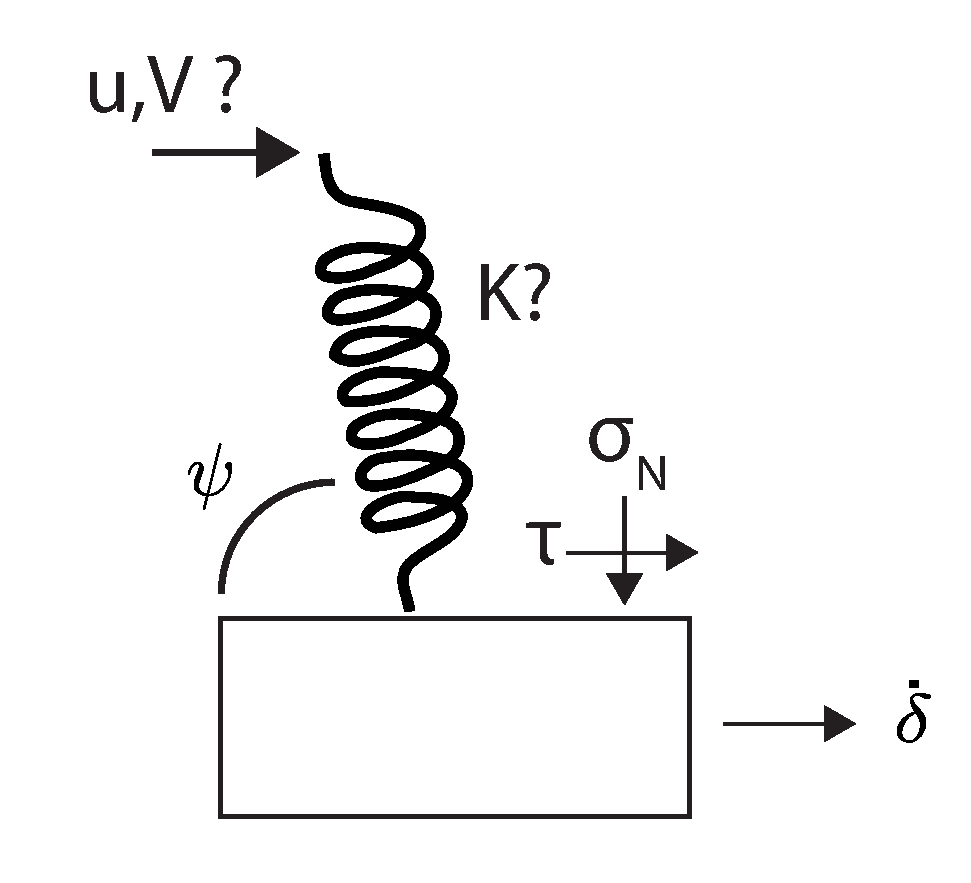
\includegraphics[width=0.25\textwidth]{Figures/D&L Stablilty High Angle Reflect.pdf}
%     \caption{A modified version of system from \citet{Dieterich1992a} at a high angle to illustrate the loose definition of the stiffness K. The sign convention for the angle follows \citet{karato2008deformation} for clarity.}
%     \label{fig:DL1992_highangle}
% \end{figure}


\section{Supplement - Full Derivations}
While the relations derived by \citet{Dieterich1992a} cover one aspect of the coupling of shear and normal stress to find a value of friction for the rate-state equation, the stiffness of the machine is ambiguously defined. Here we repeat their derivation and include the derivation of axial to shear compliance.

\begin{figure}
    \includegraphics[width=\textwidth]{Figures/Triax_Diagram_Only.pdf}
    \caption[Repeated triaxial geometry diagram]{Geometry of a triaxially confined gouge sample between two shear pistons with a schematic spring element to represent machine stiffness included. Confining stress is labeled $\sigma_3$ and axial stress is labelled $\sigma_1$. The sign convention for the angle follows \citet{karato2008deformation} instead of \citet{Dieterich1992a}.}
    \label{fig:Geometry_supp}
\end{figure}


\subsection{Derivation of Rate-State Fault Stability in Axisymmetric Saw-Cut Deformation Geometry (Triaxial)}
Rate-state friction behavior of a block slider can be described by the equations: \citep{Dieterich1992a}

\begin{equation} \label{eq:C3_S1}
    \tau =\sigma_n 
    \left(\mu_0
    +\text{Aln}\left(\frac{\dot{\delta}}{\dot{\delta}_{ss}}\right)
    +\text{Bln}\left(\frac{\theta}{\theta_0}\right)\right)
    = F\left(\dot{\delta},\theta,\sigma_n\right)
\end{equation}

\begin{equation} \label{eq:C3_S2}
    \dot{\theta}= 1
    -\frac{\theta \dot{\delta}}{D_c}
    -\frac{\alpha \theta \dot{\sigma_n}}{B \sigma_n}= G\left(\dot{\delta},\theta ,\sigma_n\right)
\end{equation}

For a confined, axially loaded piston with a plane which is rotated $\psi$ from the compression axis \citep{karato2008deformation}:

\begin{equation} \label{eq:C3_S3}
    \tau =\frac{\sigma_1-\sigma_3}{2} \sin(2\psi)
\end{equation}

\begin{equation} \label{eq:C3_S4}
    \sigma_n=\frac{\sigma_1+\sigma_3}{2}-\frac{\sigma_1-\sigma_3}{2} \cos(2\psi)
\end{equation}

Eliminating $\sigma_1$:

\begin{equation} \label{eq:C3_S5}
    \sigma_n=\sigma_3+\tau\tan(\psi)
\end{equation}

For the rest of the analysis we assume confining stress ($\sigma_3$) to be constant.
Stability analysis is performed for perturbations about a steady state:
$\tau =\tau_{ss},\text{ }
\theta =\theta_{ss},\text{ }
\dot{\delta}=\dot{\delta}_{ss}, \text{ }
\text{and }\sigma_n=\sigma_{n,ss} $
for both shear stress and state:

\begin{equation} \label{eq:C3_S6}
    \hat{\tau}= \frac{\partial F}{\partial \dot{\delta}}\dot{\hat{\delta}} + \frac{\partial F}{\partial \theta}\hat{\theta} +\frac{\partial F}{\partial
    \sigma_n}\hat{\sigma_n}
\end{equation}

\begin{equation} \label{eq:C3_S7}
    \dot{\hat{\theta}}=\frac{\partial G}{\partial \dot{\delta}}\dot{\hat{\delta}} + \frac{\partial G}{\partial \theta}\hat{\theta} +\frac{\partial
    G}{\partial \sigma_n}\hat{\sigma_n}
\end{equation}


For a block - slider type system, the shear force is balanced by force in the spring (for sign conventions see \citet{Ruina1983}) :

\begin{equation} \label{eq:C3_S8}
    \sigma_1=K_{ax}\left(v_{0,ax}t-x_{ax}+L_{ss}\right)
\end{equation}

The relation between angled fault displacement and axial displacement is:

\begin{equation} \label{eq:C3_S9}
    x_{ax}=\delta \cos{\psi}, \text{}
    v_0 = \dot{\delta}_{ss} \cos{\psi}
\end{equation}

\begin{equation} \label{eq:C3_S10}
    \sigma_1=K_{ax}\cos{\psi}
    \left( \dot{\delta}_{ss}t-\delta \right)
\end{equation}

Partial derivatives at steady state are:
\begin{equation} \label{eq:C3_S11}
    \frac{\partial F}{\partial \dot{\delta}}=\frac{\sigma_{n,ss}A}{\dot{\delta}_{ss}}
\end{equation}
\begin{equation} \label{eq:C3_S12}
    \frac{\partial F}{\partial \theta} = \frac{\sigma
    _{n,ss}B}{\theta_{ss}}
\end{equation}
\begin{equation} \label{eq:C3_S13}
    \frac{\partial F}{\partial \sigma_n}= \mu_0\
\end{equation}

State derivatives are more complex. We need to solve in terms of $\delta$ and $\theta$ so we rearrange normal stress relations in terms to substitute into (\ref{eq:C3_S2}2).

We use the time derivatives of (\ref{eq:C3_S3}3), (\ref{eq:C3_S5}5), and (\ref{eq:C3_S10}10) to find the normal stress time derivative (numerator in (\ref{eq:C3_S2}2)):
\begin{equation} \label{eq:C3_S14}
    \dot{\sigma_n}=K_{ ax}\left(\dot{\delta}_{ss}-\dot{\delta}\right)\sin(\psi)\sin(2\psi)/2
\end{equation}
Using (\ref{eq:C3_S5}5), (\ref{eq:C3_S1}1), and assuming $\theta =\theta_{ss}$ at the time we perturb the system (denominator in (2)):
\begin{equation} \label{eq:C3_S15}
    \frac{1}{\sigma_n}=\frac{1}{\sigma_3}-\frac{\tan(\psi)}{\sigma
    _3}\left(\mu_0+\text{Aln}\left(\frac{\dot{\delta}}{\dot{\delta}_{ss}}\right)\right)
\end{equation}

Then partial derivatives are:
\begin{equation} \label{eq:C3_S16}
    \frac{\partial G}{\partial \dot{\delta}}=-\frac{\theta
    _{ss}}{D_c}-\frac{\alpha \theta_{ss}}{B}K_{ ax}\sin(\psi)\sin(2\psi)\frac{\mu_0\tan(\psi)-1}{2\sigma_3}
\end{equation}

\begin{equation} \label{eq:C3_S17}
    \frac{\partial G}{\partial \theta}= -\frac{\dot{\delta}_{ss}}{D_c}
\end{equation}

\begin{equation} \label{eq:C3_S18}
    \frac{\partial G}{\partial \sigma_n}=0
\end{equation}

((\ref{eq:C3_S17}17) is unintuitive until we consider that we substituted (14) whose steady state value is 0)

We would like to solve for only the 2x2 system $\delta$ and $\theta$ so we need relationships for  $\hat{\tau} \text{ and } \hat{\sigma}$ in terms of shear displacement $\hat{\delta}$. Using (\ref{eq:C3_S3}3),(\ref{eq:C3_S5}5), and (\ref{eq:C3_S8}8):

\begin{equation} \label{eq:C3_S19}
    \hat{\tau} =K_{ax}\cos(\psi)\left(-\hat{\delta}\right) \sin(2\psi)/2
\end{equation}

\begin{equation} \label{eq:C3_S20}
    \hat{\sigma_n} =\hat{\tau}\tan(\psi),
    \hat{\sigma_n} = K_{ax}\sin(\psi)\left(-\hat{\delta}\right) \sin(2\psi)/2
\end{equation}

Using those in (\ref{eq:C3_S6}6) we get:

\begin{equation} \label{eq:C3_S21}
    K_{ax} \cos(\psi)
    \left(-\hat{\delta}\right) \sin(2\psi)/2=
    \frac{\sigma_{n,ss}A}{\dot{\delta}_{ss}}
    \dot{\hat{\delta}}
    +\frac{\sigma_{n,ss}B}{\theta_{ss}}
    \hat{\theta}
    +\mu_0 K_{ax}\sin(\psi)
    \left(-\hat{\delta}\right) \sin(2\psi)/2
\end{equation}


which reduces to
\begin{equation} \label{eq:C3_S22}
    \dot{\hat{\delta}} 
    = \frac{\dot{\delta}_{ss}}{\sigma_{n,ss}A}
    \left[
    \frac{K_{ax}\sin(2\psi)}{2}(\mu_0\sin(\psi)
    -\cos(\psi))\hat{\delta}
    -\frac{\sigma_{n,ss}B}{\theta_{ss}}
    \hat{\theta}
    \right]
    =a_{11}\hat{\delta}+a_{12}\hat{\theta}
\end{equation}

\begin{equation} \label{eq:C3_S23}
    a_{11} = 
    \frac{\dot{\delta}_{ss}}{\sigma_{n,ss}A}
    \left[
    \frac{K_{ax}\sin(2\psi)}{2}(\mu_0\sin(\psi)
    -\cos(\psi))
    \right]
\end{equation}

\begin{equation} \label{eq:C3_S24}
    a_{12} = -\frac{\dot{\delta}_{ss}B}{\theta_{ss}A}
\end{equation}


Now we can solve (\ref{eq:C3_S7}7). Note that we need to substitute for $\dot{\hat{\delta}}$:

\begin{equation} \label{eq:C3_S25}
    \dot{\hat{\theta}} 
    = \left(
    -\frac{\theta_{ss}}{D_c}
    -\frac{\alpha \theta_{ss}}{B}K_{ax}\sin(\psi)\sin(2\psi)\frac{\mu
    _0\tan(\psi)-1}{2\sigma_3}
    \right) \dot{\hat{\delta}}
    +-\frac{\dot{\delta}_{ss}}{D_c}\hat{\theta}
    =a_{21}\hat{\delta}+a_{22}\hat{\theta}
\end{equation}

\begin{equation} \label{eq:C3_S26}
    a_{21} = \left(
    -\frac{\theta_{ss}}{D_c}
    -\frac{\alpha \theta_{ss}}{B}K_{ax}\sin(\psi)\sin(2\psi)\frac{\mu
    _0\tan(\psi)-1}{2\sigma_3}
    \right)
    \frac{\dot{\delta}_{ss}}{\sigma_{n,ss}A}
    \left[
    \frac{K_{ax}\sin(2\psi)}{2}(\mu_0\sin(\psi)
    -\cos(\psi))
    \right]
\end{equation}

\begin{equation} \label{eq:C3_S27}
    a_{22} = \left(
    \frac{B-A}{D_c}+
    \alpha K_{ax}\sin(\psi)\sin(2\psi)\frac{\mu_0\tan(\psi)-1}{2\sigma_3}
    \right)
    \frac{\dot{\delta}_{ss}}{A}
\end{equation}

As \citet{Dieterich1992a} indicates, the square matrix can be solved for its eigenvalues through a quadratic characteristic polynomial. The coefficient of the second term is the trace of the matrix and controls damping so we solve for that to be 0. The system is stable above evaluated critical stiffness and unstable below evaluated critical stiffness. Note the third and fourth portions match the relation presented in \citet{Dieterich1992a}, and follow a sign convention of positive values for sawcut angle.

\begin{equation} \label{eq:C3_S28}
K_{ax,stable} \geq \frac{2}{\cos(\psi) \sin(2\psi)}\frac{\sigma_3}{1-\mu_0\tan(\psi)}\frac{(B-A)}{D_c}\frac{1}{1-\left(\mu_0-\alpha \right)\tan
(\psi)}
\end{equation}

%%
\subsection{Inter-Piston Friction}
Friction between a guided axial piston and a shear piston sliding horizontally due to compression can be included by modifying the term for confining stress to include a friction term ($\mu_r\sigma_1$) coupled to axial stress. Because no modification is made to F or G, the equations can be worked through in the same way with minor substitutions:

\begin{equation} \label{eq:C3_S29}
    \sigma_3'=\sigma_3+\mu_r\sigma_1
\end{equation}

\begin{equation} \label{eq:C3_S30}
    \sigma_n=\frac{1}{1-\mu_r}\left(\left(\mu_r\cot (\psi)+\tan(\psi)\right)\tau +\sigma_3\right)
\end{equation}

\begin{equation} \label{eq:C3_S31}
    \hat{\tau} = K_{ ax}\cos(\psi)\left(-\hat{\delta}\right)\left(1-\mu_r\right) \sin(2\psi)/2
\end{equation}

\begin{equation} \label{eq:C3_S32}
    \hat{\sigma_n} =K_{ ax}\cos(\psi)\left(-\hat{\delta}\right) \left(1-\cos(2\psi)+\mu_r(1+\cos(2\psi))\right)/2
\end{equation}

\begin{equation} \label{eq:C3_S33}
    \sigma_{n,ss}=\frac{\sigma_3}{1-\mu_r-\mu_0\left(\mu_r\cot (\psi)+\tan(\psi)\right)}
\end{equation}

\begin{equation} \label{eq:C3_S34}
    K_{ ax} \geq \frac{2}{\cos(\psi)}\sigma_{n,ss}\frac{(B-A)}{D_c}\frac{1}{\left(1-\mu_r\right)\sin(2\psi)-\left(\mu_0-\alpha \right)\left(1-\cos
    (2\psi)+\mu_r(1+\cos(2\psi))\right)}
\end{equation}

This is greater (less stable) than (\ref{eq:C3_S15}15) with $\mu_r>0$, and reduces to (\ref{eq:C3_S15}15) when $\mu_r=0$. In practice the piston contact friction may be larger than bending stiffness of axial forcing rods so this may not be dominant in all cases.

%%
\subsection{Confining Resistance}
Another potential source of stabilization is resistance on the shear pistons expanding into the confining media. The resistance could be metal jacket stretching or deformation of the confining media. The formulation is simplified as a general linear velocity dependent resistance $\eta$ with scale included.
\begin{equation} \label{eq:C3_S35}
    \sigma_3'=\sigma_3+\eta\dot{\delta}\sin(\psi)
\end{equation}

\begin{equation} \label{eq:C3_S36}
    \sigma_n=\sigma_3+\eta \dot{\delta}\sin(\psi)+ \tau\tan(\psi)
\end{equation}

\begin{equation} \label{eq:C3_S37}
    \hat{\tau} =\frac{1}{2}\sin(2\psi)\left(K_{ ax}\cos(\psi)\left(-\hat{\delta}\right)+\eta  \sin(\psi)\left(-\dot{\hat{\delta}} \right)\right)
\end{equation}

\begin{equation} \label{eq:C3_S38}
    \hat{\sigma_n} =\frac{1}{2}
    \left(
        (1-\cos(2\psi))K_{ax}\cos(\psi)
        \left(-\hat{\delta}\right)
        +(1+\cos(2\psi))\eta\sin(\psi)
        \left(\dot{\hat{\delta}}\right)
    \right)
\end{equation}

\begin{equation} \label{eq:C3_S39}
    \dot{\sigma_n} = K_{ax}\left(\dot{\delta}_{ss}-\dot{\delta}\right)\sin(\psi)\sin(2\psi)/2+\eta\Ddot{\delta}\sin(\psi)\cos^2(\psi)
\end{equation}

\begin{equation} \label{eq:C3_S40}
    \frac{1}{\sigma_n} = \frac{1-\tan(\psi)\left(\mu_0 +\text{Aln}\left(\frac{\dot{\delta}}{\dot{\delta}_{ss}}\right)\right)}{\sigma_3+\eta\dot{\delta}\sin(\psi))}
\end{equation}

Here we assume that resistance is a secondary effect so the resistance term containing $\Ddot{\delta}$ is small and can be neglected.

\begin{equation} \label{eq:C3_S41}
    \frac{\partial G}{\partial \dot{\delta}}=-\frac{\theta_{ss}}{D_c}-\frac{\alpha \theta_{ss}}{B}k_{ ax}\sin(\psi)\sin(2\psi)\frac{\mu_0\tan(\psi)-1}{2(\sigma_3+\eta\dot{\delta}_{ss}\sin(\psi))}
\end{equation}

\begin{equation} \label{eq:C3_S42}
    \sigma_{n,ss}=\frac{\sigma_3+\eta \sin(\psi)\dot{\delta}_{ss}}{1-\mu_0\tan(\psi)}
\end{equation}

\begin{equation} \label{eq:C3_S43}
K_{ax} \geq 
\frac{1}{\cos(\psi)\sin(2\psi)}\frac{1}{(1-(\mu_0-\alpha)\tan(\psi))}
\frac{1}{D_c}
\left(2\sigma_{n,ss}(B-A) -\mu_0\eta\dot{\delta}_{ss}\sin(\psi)(1+\sin(2\psi)+\cos(2\psi))\right)
\end{equation}

The derived stiffness is lower (more stable), with the magnitude of the change roughly proportional to the ratio $\mu_0\eta\dot{\delta}_{ss}:2\sigma_{n,ss}(B-A)$. 

%%
\subsection{Shear Viscous Resistance}
Another relevant scenario to consider is viscous support of the sample (Kelvin-Voight like), where a generalized velocity dependent term is added to shear stress, F. This doesn't change any of the geometric relationships, only the partial derivative of F and steady state. The schematic representation could be a fault with viscous patches or resistance that only generates shear traction (such as drag along the sides of shear pistons):
\begin{equation} \label{eq:C3_S44}
\tau =\sigma_n \left(\mu_0+\text{Aln}\left(\frac{\dot{\delta}}{\dot{\delta}_{ss}}\right)+\text{Bln}\left(\frac{\theta}{\theta_0}\right)\right)+\eta\dot{\delta}=F\left(\dot{\delta},\theta ,\sigma \right)
\end{equation}

\begin{equation} \label{eq:C3_S45}
\frac{\partial F}{\partial \dot{\delta}}=
\frac{\sigma_{n,ss}A}{\dot{\delta}_{ss}} +\eta
\end{equation}

\begin{equation} \label{eq:C3_S46}
\sigma_{n,ss}=\frac{\sigma_3+\eta  \dot{\delta}_{ss}\tan(\psi)}{1-\mu_0\tan(\psi)}
\end{equation}

\begin{equation} \label{eq:C3_S47}
K_{ ax} \geq \frac{1}{\cos(\psi)\sin(2\psi)}\frac{1}{1-(\mu_0-\alpha)\tan(\psi)}\frac{1}{D_c}\left(2\sigma_{n,ss}(B-A) -2\eta \dot{\delta}_{ss}\right)
\end{equation}

No extra angular terms are present in the resulting stability condition because the resistance directly opposes fault motion regardless of direction and does not depend on normal stress.  Steady-state normal stress decreases with decreasing fault angle so at low fault angles the resistance term can be larger and completely stabilize the system.

\subsection{Normal Faults}
Normal faults will be addressed here without rotating geometry because stiffness is defined for axial stress $\sigma_1$. An extensional fault would have axial stress lower than confining stress, causing the friction coefficient to be negative. Rate dependence A and B do not change. The result is much lower required stiffness for stability at high fault angles due to reduced normal stress.

The external effects can also be addressed with the change in sign required for confining viscosity and inter-piston friction (forces resist direction of movement). 
\begin{enumerate}
    \item Inter-piston friction mildly stabilizes the fault at high angles due to normal stress reduction, but causes locking at very low angles.
    \item Confining resistance strongly stabilizes the fault by effectively reducing normal stress.
    \item Viscous shear effects stabilize the fault for the same reasons at high stress as low stress. The difference between extension and compression at high angles is the magnitude of the frictional shear stresses (small in extension, large in compression).
\end{enumerate}



%%
\subsection{Piston Offset}
The triaxial piston geometry has a significant limitation in that area of contact changes for slipping pistons with displacement. The area change can be calculated by measuring the cross-correlation of two circles (or ellipses) offset by a fraction of their diameter $d_0$. For an angled sawcut overlap this is calculated as:
\begin{equation} \label{eq:C3_S48}
    s(\delta)=\frac{\delta}{d_0/\sin{\psi}}
\end{equation}

The area fraction can then be calculated as:

\begin{equation} \label{eq:C3_S49}
    f(s) = \frac{\text{Area}}{\text{Area}_0}= 1 - 1.2082 {s} - 0.19134 {s}^2 + 0.39461 {s}^3
\end{equation}

We refer to this function as $f(s(\delta))$. For two squares (direct shear) the function is $1-s$. The area correction causes stress to increase with increasing displacement even though apparent force is decreasing. 

At any time given a load (fault shear stress $\tau$ here) there will be an increase in effective load due to area reduction and a decrease in applied load due to spring unloading. The magnitude of these two contributions changes with displacement.

In a simple case where steady-state load is fixed:
\begin{equation} \label{eq:C3_S50}
    K_{\tau,s}=\frac{d\tau_{spring}}{ds}=\frac{d\tau}{dF}\frac{dF}{dx}\frac{dx}{d\delta}\frac{d\delta}{ds}=K_{ax}*\frac{\sin{2\psi}}{2}\cos{\psi}\frac{d_0}{\sin{\psi}}
\end{equation}
\begin{equation} \label{eq:C3_S51}
    K_{\tau,s, unloading}=K_{\tau,s}/f(s)
\end{equation}

\begin{equation} \label{eq:C3_S52}
    \tau_{eff}=\tau_{ss}/f(s)
\end{equation}
\begin{equation} \label{eq:C3_S53}
    \frac{d\tau_{eff}}{ds}=\tau_{ss}*\frac{-1}{f^2}\frac{df}{ds}
\end{equation}

\begin{equation} \label{eq:C3_S54}
    K_{obs} = -K_{\tau,s, unloading}+\frac{d\tau_{eff}}{ds}
\end{equation}

These two terms have opposite signs (load decrease and increase, respectively) so they compete to control stability over fault displacement. Fixed variables are spring stiffness, fault length, fault angle, and $\sigma_3$. Note that long faults are inherently more stable here ($d_0/\sin{\psi}$).
Also note how the effective fault stiffness is affected by current load in the latter set of equations $\tau_{control}$. This dependence on current load will cause slipping faults to stabilize if stiffness is high.

For the particular case of relaxation, stress evolves as:
\begin{equation} \label{eq:C3_S55} %no double counting here
    \tau_{elastic}(s)=\tau_{0}-K_{\tau,s}*s
\end{equation}
\begin{equation} \label{eq:C3_S56}
    \tau_{eff}=\tau_{elastic}(s)/f(s)
\end{equation}
\begin{equation} \label{eq:C3_S57}
    \frac{d\tau_{eff}}{ds}(s)=\tau_{elastic}(s)*\frac{-1}{f^2}\frac{df}{ds}-K_{\tau,s}/f(s)
\end{equation}
Many cases are more stable than constant stress because spring/applied stress is much lower at large displacement.



%%%
\section{Apparatus Application}
\citet{Okazaki2015} observe stick-slip in antigorite at 250 MPa confining pressure, with shear stiffness of 58 MPa/mm, a steady state friction coefficient of 0.7 and a saw-cut piston angle of 30 degrees. A-B is -0.005 with a transition to the relevant negative values above 500C. \citet{Proctor2015} do not observe stick-slip at 1000 MPa confining pressure with axial stiffness of 2 GPa/mm, steady-state friction coefficient of 0.4 and a saw-cut piston angle of 45 degrees. \citet{burdette2020enhanced} observe shear heating, but no unstable-stick slip under the same conditions as Proctor and Hirth (2015) with axial stiffness reduced by an order of magnitude.

\begin{figure}[ht]
      \includegraphics[width=\textwidth]{Figures/Okazaki_Burdette_example.png}
      \caption[Comparison of required stiffness in Okazaki]{Plot of required machine stiffness for stable sliding of gouge between saw-cut pistons in triaxial compression. The blue line was determined using parameters from \citet{Okazaki2015} ($\mu_0=0.7, A-B=-0.005, Dc=55\mu m, \sigma_3=250 MPa)$, and the blue point is at the conditions of 600C experiments showing slow-slip. The orange line (higher up in the figure) was calculated with measured friction and confining pressure from \citet{Proctor2015} ($\mu_0=0.5, \sigma_3=1000 MPa$). Orange Dots correspond to run conditions of standard stiffness experiments of Proctor and Hirth (2015), and reduced stiffness experiments of Burdette and Hirth (2020).}
    \label{fig:Example}
\end{figure}

\end{document}
